% !TEX TS-program = XeLaTeX
% use the following command: 
% $ xelatex -shell-escape -output-driver="xdvipdfmx -z 0" article.tex
% this "-z 0" must be used to suppress compression in XMP Metadata packet 
% all document files must be coded in UTF-8
\documentclass{textolivre}
% for anonymous submission
%\documentclass[anonymous]{textolivre}
% to create HTML use 
%\documentclass{textolivre-html}
% remove all auxiliary files
% find . -name 'tl-article-template.*' ! -name '*.tex' ! -name '*.pdf' ! -name '*.bib' -type f -exec rm {} \;
% HTML compile using make4ht
% $ make4ht -c textolivre-html.cfg -u -x article "fn-in,svg"   # or use `mathjax' instead of `svg' to get LaTeX equation that will be handled by MathJax
% $ bibtex article
% clean and prettify HTML 
% $ tidy -o article-tidy.html --output-xhtml --break-before-br --wrap 0 article.html 2> errs.txt
% https://www.html-tidy.org/documentation/

% Metadata
\begin{filecontents*}{article.xmpdata}
    \Title{Análisis de los nuevos anglicismos léxicos en la lengua española en el contexto de las obras y corpus académicos digitales}
    \Author{David Giménez Folqués}
    \Language{es}
    \Keywords{Anglicismos \sep Corpus acadêmicos \sep Dicionários acadêmicos \sep Lexicologia \sep Lexicografia}
    \Journaltitle{Texto Livre}
    \Journalnumber{1983-3652}
    \Volume{14}
    \Issue{1}
    \Firstpage{1}
    \Lastpage{16}
    \Doi{10.35699/1983-3652.2021.24418}

    \setRGBcolorprofile{sRGB_IEC61966-2-1_black_scaled.icc}
            {sRGB_IEC61966-2-1_black_scaled}
            {sRGB IEC61966 v2.1 with black scaling}
            {http://www.color.org}
\end{filecontents*}

% - install package icc-profiles
% - it is necessary to convert all image files to PDF/A
%   use ghostscript as shown below:
%   PDF images:
%   $ gs -dPDFA -dBATCH -dNOPAUSE -sColorConversionStrategy=UseDeviceIndependentColor -dCompatibilityLevel=1.4 -sDEVICE=pdfwrite -sProcessColorModel=DeviceCMYK -dPDFACompatibilityPolicy=2 -sOutputFile=figure-a.pdf figure.pdf
%   Other images:
%   $ convert figure.png figure.eps
%   $ gs -dPDFA -dBATCH -dNOPAUSE -sColorConversionStrategy=UseDeviceIndependentColor -dCompatibilityLevel=1.4 -sDEVICE=pdfwrite -sProcessColorModel=DeviceCMYK -dPDFACompatibilityPolicy=2 -dEPSCrop -sOutputFile=figure.pdf figure.eps

\journalname{Texto Livre: Linguagem e Tecnologia}
\thevolume{14}
\thenumber{1}
\theyear{2020}
\receiveddate{\DTMdisplaydate{2020}{08}{01}{-1}} % YYYY MM DD
\accepteddate{\DTMdisplaydate{2020}{08}{17}{-1}}
\publisheddate{\DTMdisplaydate{2020}{10}{15}{-1}}
% Corresponding author
\corrauthor{David Giménez Folqués}
% DOI
\articledoi{10.35699/1983-3652.2021.24418}
% Abbreviated author list for the running footer
\runningauthor{Folqués}


\title{Análisis de los nuevos anglicismos léxicos en la lengua española en el contexto de las obras y corpus académicos digitales}
\othertitle{Análise dos novos anglicismos léxicos na língua espanhola no contexto das obras e corpus acadêmico digital}
\othertitle{Use of new lexical anglicisms in the spanish through academic works and digital corpus}
% if there is a third language title, add here:
%\othertitle{Artikelvorlage zur Einreichung beim Texto Livre Journal}

\author[1]{David Giménez Folqués \orcid{0000-0002-9059-5591} \thanks{Email: \url{david.gimenez-folques@uv.es}}}
\affil[1]{Universidad de Valencia, Espanha.}

%\usepackage[backend=biber,style=abnt, ittitles]{biblatex}
%\DeclareLanguageMapping{brazil}{brazil-apa}
\addbibresource{article.bib}     
% use biber instead of bibtex
% $ biber tl-article-template
% $ pdflatex tl-article-template.tex

% set language of the article
\setdefaultlanguage{spanish}
\setotherlanguage{portuguese}
\setotherlanguage{english}

\begin{document}
% set language of the article
\maketitle

\begin{polyabstract}
\begin{abstract}
Con la llegada del siglo XXI, las obras académicas en español empezaron a mostrar un mayor interés por el anglicismo léxico, reflejando así el uso generalizado que sociedad y medios de comunicación hacían de él. Paralelamente, la accesibilidad que supone la digitalización de corpus académicos, como el CREA y el CORPES XXI de la Real Academia Española, permite investigar la progresión de estas voces en los textos que los componen. Durante los últimos años, estos anglicismos se han ajustado a las necesidades de la lengua española tanto en España como en América, bien incorporando términos, bien adaptándolos o bien rechazando aquellos que se consideraban ya inservibles. A partir de esta premisa se centra la presente investigación en tres objetivos claros; en primer lugar, mediante los corpus digitales académicos y mediante la última edición del Diccionario de la lengua española, se observa qué nuevos anglicismos han sido incluidos con respecto a la anterior edición y con qué tipología de adaptación. En segundo y tercer lugar, se analiza si se cumplen los criterios de frecuencia de uso, por un lado, y si se contempla el parámetro de necesidad frente a las voces que ya tenían equivalente patrimonial.

\keywords{Anglicismos \sep Corpus académicos \sep Diccionarios académicos \sep Lexicología \sep Lexicografía.}
\end{abstract}

\begin{portuguese}
\begin{abstract}
Com a chegada do século 21, as obras acadêmicas em espanhol passaram a mostrar um maior interesse pelo anglicismo lexical, refletindo assim o uso generalizado que a sociedade e a mídia fizeram dele. Ao mesmo tempo, a acessibilidade que implica a digitalização de corpus acadêmicos, como CREA e CORPES XXI, da Real Academia Espanhola, permite investigar a progressão dessas vozes nos textos que as compõem. Nos últimos anos, esses anglicismos se ajustaram às necessidades da língua espanhola tanto na Espanha como na América, seja incorporando termos, adaptando-os ou rejeitando aqueles que já eram considerados inúteis. Com base nessa premissa, a presente pesquisa concentra-se em três objetivos claros: primeiramente, por meio do corpus digital acadêmico e da última edição do Diccionario de la lengua española, observam-se quais novos anglicismos foram incluídos em relação à edição anterior e com que tipo de adaptação; em segundo e terceiro lugar, analisam-se os critérios de frequência de uso são atendidos, por um lado, e se o parâmetro de necessidade é considerado frente a vozes que já possuíam equivalente patrimonial.

\keywords{Anglicismos \sep Corpus acadêmicos \sep Dicionários acadêmicos \sep Lexicologia \sep Lexicografia.}
\end{abstract}
\end{portuguese}

\begin{english}
\begin{abstract}
Since the beginning of the 21st century, academic papers on Spanish linguistics have increasingly focused on collecting and classifying foreign words used in modern Spanish, reflecting their use in society, especially in contexts such as the media. Among these words there is a strong presence of Anglicisms, a fact reflected in the CREA and CORPES XXI digital corpora of the Royal Spanish Academy (RAE) and, consequently, in academic works. During the second decade of this century, these Anglicisms have gradually been adapted to the needs of the Spanish language. The present study focuses on this phenomenon, using the aforementioned corpora and the latest edition of the Diccionario de la lengua española (official Spanish dictionary of the RAE and the ASALE) to ascertain and elucidate the current situation of these Anglicisms in Spanish. In addition, it will be observed if these Anglicisms appear due to the factors of frequency and lexical need.

\keywords{Anglicisms \sep Academic corpora \sep Academic dictionaries \sep Lexicology \sep Lexicography.}
\end{abstract}
\end{english}

% if there is another abstract, insert it here using the same scheme
\end{polyabstract}


\section{Introducción}\label{sec-intro}
En las últimas décadas la lengua inglesa continúa imparable en su condición de idioma de comunicación entre culturas, lo que provoca que el trasvase de voces prolifere en otras lenguas como la española. Factores como la globalización, la progresión de Internet, la difusión de los medios de comunicación, o el uso de este idioma como lengua franca en ámbitos como los avances tecnológicos, entre otros, han provocado que el inglés mantenga esta posición dominante.

Esta influencia ocupa todas las zonas donde el español es lengua nativa, como así sucede en España y Latinoamérica; aunque no hay que olvidar el caso de Estados Unidos, donde el español se encuentra en contacto directo con el inglés. Hay que precisar que, pese a que el impacto del inglés está generalizado en la lengua española, existen zonas donde su influencia es todavía mayor, como sucede en Puerto Rico, donde el inglés es lengua oficial, o el recién citado Estados Unidos, donde, además, es posible encontrar situaciones de bilingüismo. 

Mediante este contacto lingüístico, se ha producido una transmisión de voces desde la lengua inglesa al español. En cuanto a la denominación de estas voces resultantes, centrándonos en el aspecto léxico, encontramos una clara coincidencia en el uso de la etiqueta “anglicismo”. De este modo, la última edición del Diccionario de la lengua española \cite{real2014diccionario} usa la entrada “anglicismo”\footnote{
Aunque es cierto que este término aparece ligado a una perspectiva estrictamente lingüística, como ha venido sucediendo en la tradición hispánica. Entre otras alternativas, se puede optar por un término más amplio que incluya otras disciplinas, como sería el caso de “préstamo”, empleado, entre otros, por Gómez Capuz (2009).
}y la define como “vocablo o giro de la lengua inglesa empleado en otra\footnote{
\url{ttps://dle.rae.es/?id=2eG56Yz}
}”. Igualmente, \textcite[p. 277]{amador2015} incluye el mismo término y lo define como “voces de procedencia inglesa que otras lenguas adoptan [...]”. Por su parte, \textcite{capuz2000}, además de emplear el mismo vocablo, destaca la transferencia de elementos léxicos sobre otros ámbitos como el sintáctico, por lo que resulta el fenómeno más visible y productivo si queremos observar su incidencia en la lengua española.

Asimismo, \textcite{lorenzo1987} realiza una división de este tipo de voces ciñéndose a su grado de integración en la lengua española, donde destacan aquellos anglicismos crudos que mantienen la grafía inglesa y la pronunciación próxima a este idioma y, por otro lado, aquellos que se han adaptado a las características de la lengua española. Como veremos más adelante, este criterio también es compartido por los recursos lexicográficos de la Real Academia Española y la Asociación de Academias de la Lengua Española, donde se incluyen nuevos extranjerismos\footnote{
Etiqueta usada por la RAE y ASALE para aquellas voces que proceden de una lengua distinta del español.
} en su voz original y marcados ortotipográficamente con cursiva, y aquellas nuevas voces que se integran ya adaptadas a la lengua española y en letra redonda.

Por ende, resulta obvio que el término “anglicismo” es aceptado por la mayoría de la tradición hispánica a lo largo del siglo XX y XXI y aparece documentado en español por primera vez en 1784 \cite[p. 13]{Lorenzo1996}. Sin embargo, como señala \textcite[p. 99]{RodrguezMedina2000}: “hay que trasladarse a 1948 para encontrar el primer tratado relevante dedicado en su totalidad al estudio del anglicismo en el mundo hispánico: "El anglicismo en el español contemporáneo", del abogado panameño R. Alfaro”.  A finales del siglo XX, aumentan los trabajos sobre este fenómeno, donde destacamos obras como las de \textcite{pratt1980,lorenzo1987,Lorenzo1996,medina1996,salavador1994,rodriguez1997,riquelme1998,capuz1998}, por citar solo algunas relevantes en este campo de estudio. Estas investigaciones continúan desarrollándose y se asientan en la actualidad en publicaciones como \textcite{navarro2006,capuz2009,rodriguez2013,rodriguez2017,rodriguez2018,rodriguez2019,amador2014,amador2015,moreno2018,moreno2018b}.

Por otro lado, autores como Schmidt y Diemer (2015) señalan que la recepción del anglicismo en la lengua española ha tenido diferentes acogidas y las clasifica en tres perspectivas fundamentales, una más extrema que rechaza la llegada masiva de estas voces en defensa de las voces patrimoniales, una segunda visión inclusiva, que contemplaría la riqueza que supondría su integración en el vocabulario español y una tercera equilibrada. En esta última perspectiva, pese a que no se negaría la llegada de voces inglesas, se integrarían de una manera precavida, ordenada y justificada.

Pese a que en muchos ámbitos se considera que en la actualidad la Real Academia Española (RAE), en colaboración con la Asociación de Academias de la Lengua Española (ASALE), tiene una actitud purista frente a los extranjerismos, realmente se encontraría en una situación intermedia, ya que aunque es cierto que en sus orígenes sí guardaba una actitud más bien extrema y todavía en la actualidad defiende la presencia de la voz patrimonial sobre la foránea, desde hace décadas no excluye la llegada de nuevos extranjerismos, siempre que se cumplan los parámetros de funcionalidad, frecuencia de uso, temporalidad y extensión geográfica. En esta dirección, aunque el fenómeno del anglicismo en español no es nuevo, en los últimos años, estos organismos se han preocupado de recoger y clasificar este caudal léxico de manera ordenada y justificada para evitar, entre otras cuestiones, las diversas variaciones y usos que en la sociedad estaban apareciendo. 

Junto a la RAE, toma un papel fundamental la ASALE en el nuevo rumbo que está tomando la lengua española. Mediante la aparición e influencia de este nuevo organismo, se incluyen más voces procedentes de América en las obras académicas, como podemos constatar, entre otros, en \textcite{morales2006} o \textcite{martin2009}. Por lo tanto, también se amplía el abanico para las voces foráneas que son usadas en este continente en el idioma español, entre ellas, evidentemente, los anglicismos.

La RAE se crea en 1713 en Madrid, mientras que en el siglo XIX se origina la creación de las academias de los distintos países latinoamericanos. En 1951 aparece en México la ASALE, en la que actualmente participan las 24\footnote{
Contamos con 24 Academias de la Lengua Española, ya que recientemente se han unido la Academia Ecuatoguineana de la Lengua Española (2013) y la Academia Nacional del Ladino (2018).
} academias donde el español es nativo o tiene mucha relevancia. Uno de los objetivos de estos organismos es el de velar por la uniformidad del idioma manteniendo una normativa pluricéntrica\footnote{
La posibilidad de este carácter pluricéntrico se origina en el intento de que todas las variedades se sientan representadas en las diferentes obras académicas. Este objetivo adquiere mayor relevancia a partir de la creación de la ASALE.
}.

En 1780 ve la luz lo que se considera como la primera edición del diccionario de la lengua española de la RAE en un único tomo\footnote{
Edición en un único tomo del Diccionario de autoridades publicado entre 1726 y 1739 (REAL ACADEMIA ESPAÑOLA).
}. Desde entonces, hemos observado la aparición de 23 ediciones de diccionarios, siendo el 2014 la fecha de la 23.ª edición, donde los neologismos y el contacto lingüístico siempre han estado presentes, como señala \textcite[p. 276]{amador2015}:

\begin{quote}
Durante el siglo XVIII aparecieron tres ediciones; en el siglo XIX fueron diez, entre las que destacan la edición de 1803, caracterizada por la admisión de numerosos neologismos científicos; y la de 1884, en la que se admiten diversas voces técnicas y del habla popular y comienzan a incluirse las etimologías el léxico procedente de otros países hispanohablantes. En el siglo XX se publicaron ocho, siendo la más relevante la de 1925, edición en que se registra un considerable aumento de americanismos. En el siglo XXI han sido publicadas dos ediciones, la de 2001 que incluye gran cantidad de voces del español de América y la de 2014.
\end{quote}

Aunque es cierto que desde los inicios del Diccionario podemos encontrar neologismos, los extranjerismos fueron repudiados en sus primeras ediciones. Se era consciente de que estas voces foráneas se estaban utilizando en la sociedad, sin embargo, se evitaron hasta la llegada de la edición de 1884, la que correspondería a la 12.ª edición del Diccionario. En ese momento se incluyen muchas de aquellas voces que ya circulaban anteriormente entre los hablantes de español.

La incorporación de anglicismos es un fiel reflejo del criterio de inclusión que acabamos de mencionar, junto con la mayor influencia de la lengua inglesa en la sociedad durante las últimas décadas. En este sentido, \textcite{pedrero2007} resume la llegada de anglicismos en el Diccionario en cuatro fases. Una primera fase, de 1780 a 1852, donde apenas se incluyen 6 anglicismos; una segunda fase, de 1869 a 1899, donde ya se incluyen 81 voces; una tercera fase, de 1914 a 1947, con 63 nuevos anglicismos y una cuarta fase, hasta la 22.ª edición, donde el número resulta mucho más notorio, con un total de 509 nuevas voces.

Por lo tanto, en estas últimas décadas, la llegada de extranjerismos y, en concreto, de anglicismos, cada vez es mayor. En este camino resulta fundamental la publicación del Diccionario panhispánico de dudas (DPD) en el año 2005, obra que incluye un gran número de anglicismos, en su forma original y adaptadas al español, debido a la preocupación existente en la RAE y ASALE sobre las diferentes variantes existentes, como es el caso de “básket, basketball, básketbol, basketbol, baloncesto, básquetbol, basquetbol”, o el de “vóley, volleyball, vóley-playa, voleibol, vóleibol, voleybol”. A partir de esta variación, la obra realiza propuestas para seleccionar la forma adecuada y, también, su pronunciación. En cuanto a los anglicismos léxicos, la RAE y la ASALE diferencian entre los necesarios y los innecesarios. Los necesarios son aquellos que no cuentan con un equivalente patrimonial en la lengua española, como sería el caso de “jazz” o de “jacuzzi”; mientras que los innecesarios sí contarían ya con un equivalente léxico, como sería el caso de “baby sitter” con “niñera” o el de “show” con “espectáculo”. En este sentido, el criterio que aplican estos organismos es el de adaptar al español aquellas voces foráneas que no tienen un equivalente patrimonial y, en segundo lugar, aconsejar el uso del equivalente español en los anglicismos que sí disponen de él.

Como podemos ver, a excepción de los extranjerismos originales extendidos en la sociedad, el objetivo es obtener una forma lingüísticamente “española”, ya sea por la adaptación del anglicismo o por el consejo de usar su equivalente. En esta dirección han trabajado la RAE y la ASALE en la última edición del Diccionario de la lengua española (2014), donde se han eliminado algunos anglicismos que tenían un equivalente español, como “hit” y su adaptación “jit”, en favor de “(gran) éxito”; y otros se han mantenido adaptados por carecer de tal equivalente, como es el caso de “brandi”, “curri” o “kétchup”.

Un aspecto fundamental en la elaboración del DPD o el DLE son los corpus académicos. Estos corpus aparecen en formato digital, con lo cual su accesibilidad es mayor para los usuarios de la lengua. Durante finales del siglo XX, el CREA (Corpus de Referencia del Español Actual) fue la referencia de la que se nutrían las obras académicas como el Diccionario de la lengua española en su 22.ª edición (2001). Este corpus digital recoge textos desde el año 1975 hasta el 2004, siendo una de las primeras referencias de lo que conocemos como el español actual. Incluye todas las variedades del español y diferentes formatos de texto, tanto escritos como orales y en diferentes temáticas. En la mencionada 22.ª edición\footnote{
Pese a la amplia recogida de anglicismos en esta edición del \emph{Diccionario}, \textcite{mejias2002} señala que tendrían que revisarse en las siguientes ediciones los apartados de etimologías, envíos y definiciones, debido a la gran cantidad de errores que encontramos en ellos.
} del Diccionario ya se incorpora un gran número de anglicismos con respecto a las ediciones anteriores, es decir, 117 nuevas voces procedentes de la lengua inglesa debido a su importancia en ámbitos como la tecnología, la ciencia, el deporte o los medios de comunicación. 

En la actualidad, el corpus vigente es el CORPES XXI (Corpus del Español del Siglo XXI).  Este último corpus digital representa la base de la última edición del Diccionario de la lengua española (edición 23.ª, con fecha del 2014). También recoge textos de toda índole, en medios escritos, y orales y representa a las diferentes variedades del español\footnote{
70\% de textos pertenecientes a Latinoamérica y 30\% a España.
}. 

En definitiva, en el presente trabajo nos disponemos a abordar tres objetivos claros a partir del contexto que acabamos de analizar. En primer lugar, contemplaremos el objetivo intrínseco de observar qué anglicismos se han incluido en la 23.ª edición del Diccionario de la lengua española \cite{real2014diccionario} en contraste con la 22.ª edición de la obra \cite{real2001diccionario} y, consecuentemente, analizaremos lingüísticamente los métodos de adopción y adaptación que han experimentado estas voces durante su inclusión. En segundo lugar, observaremos si la incorporación de estos nuevos anglicismos por parte de la RAE y la ASALE responde al criterio de frecuencia de uso mediante el filtro de los corpus académicos digitales CREA y CORPES XXI. La frecuencia de aparición en los textos españoles recogidos en estos corpus académicos indicaría que los anglicismos incluidos como novedosos realmente responden a una necesidad social de uso. Finalmente abordaremos el criterio de necesidad léxica tan marcado en la RAE en la recogida de extranjerismos. Mediante la inclusión de anglicismos con o sin equivalente patrimonial observaremos no solo el tipo de anglicismos que se está contemplando, extranjerismo necesario o innecesario, sino también el rumbo que están tomando los organismos académicos en este sentido.



\section{Metodología de análisis}\label{sec-metodologia}
Para desarrollar la presente investigación utilizaremos como fuentes principales de extracción de anglicismos las dos últimas ediciones del Diccionario de la lengua española para comprobar, de este modo, qué anglicismos han sido incluidos en la última edición del 2014.

En segundo lugar, a partir del caudal léxico resultante, analizaremos los corpus digitales CREA y CORPES XXI (REAL ACADEMIA ESPAÑOLA) para observar si la RAE y la ASALE han seguido el factor de frecuencia de uso para la inclusión de estas voces. Es decir, si los hablantes de la lengua española las han usado y si, a su vez, cubren vacíos léxicos, por lo que incluiremos, en el caso de que aparezca, su equivalente vigente en español\footnote{
El equivalente suele venir sugerido por el DLE \cite{real2014diccionario}. En muchas ocasiones, existen equivalentes léxicos en español que son desechados en favor del anglicismo. Sin embargo, la RAE y la ASALE siguen recomendando, mientras exista, este equivalente en español.
}. Este factor de necesidad nos permitirá clasificar mejor los anglicismos resultantes y la influencia que puede conllevar en su fisionomía ortográfica final ante una posible adaptación o no. Para todo ello elaboraremos fichas lexicográficas que nos permitan alcanzar un aspecto visual y comparativo. En estas fichas incluiremos los apartados “voz”, “definición en DLE (23.ª edición)”, “año de inclusión en los corpus”, “frecuencia de aparición en CREA”, “frecuencia de aparición en el CORPES XXI” y “equivalente en español”, si es el caso. Mediante la inclusión de los dos corpus observaremos la progresión de estas voces en frecuencia, además del momento exacto de incorporación en los textos recogidos. Por otro lado, computaremos el porcentaje de anglicismos necesarios e innecesarios mediante la pestaña “equivalente en español”.

Asimismo, si en la búsqueda de casos en el CREA o CORPES XXI el anglicismo presenta variaciones de género o número, estos también serán incluidos en los resultados de frecuencia de uso, ya que se consideran parte del mismo fenómeno de adaptación. Por otro lado, únicamente incluimos los resultados que tienen que ver con el significado señalado en la definición de la ficha, por lo que se desecha el resto.

Finalmente, analizaremos lingüísticamente la adopción y adaptación de estas voces a la lengua española. Es decir, precisaremos qué tipo de anglicismos predominan en su inclusión en la última edición del Diccionario y qué métodos lingüísticos de adaptación han sido las más frecuentes a la hora de llevarlos a cabo.



\section{Nuevos anglicismos en DLE (23.ª edición)}\label{sec-anglicismos}
A continuación, vamos a enumerar alfabéticamente los nuevos anglicismos que añade y propone el DLE en su 23.ª edición en relación con la anterior. Respetaremos su aparición ortotipográfica en el DLE, por lo que las voces adaptadas a la lengua española se incluirán en letra redonda y las voces originales o crudas en cursiva. Asimismo, si existen variantes sobre la misma voz estas también serán contempladas:

Acid (acid house y acid jazz); antidumping; ataché; autólogo/a; backgammon; backstage; beat; beatnik; bioenergía; birdie; blackjack/black jack/black-jack; bloguero/a; blue jean; bodi; bogey; bogie, bótox; boy scout; brandi; break; break dance; bridge; brik/tetrabrik; buldócer; bungaló; cartoon; catch; chill out; clicar/cliquear/cliqueo; coach; container; copyright; country; cracker; crash; críquet; cuark; cuásar; curri; dron; eagle; escúter; espanglish; especismo/especista; espray; esprint; establishment; estand; estriptis/estriptís; euríbor; fair play; ferri; finger; full; giga; gigabyte; ginseng; hackear; hacker; heavy; holter; intranet; jean; jeep; jet lag; jumbo; kilobyte; megabyte; órsay; panti; parking; party; performance; pinqui; playback; playboy; pop art; pósit; pub; puenting; quad; rafting; reality; remake; rocanrol; serendipia; sex shop; sex symbol; sexi; show business; showman; sketch; spa; spam; sparring; squash; stent; stop; superwoman; swing; táper; terabyte; thriller; tie break; tofe; top model; trávelin; tuit/tuitear/tuiteo/tuitero-a; tunear; tweed; twist; underground; walkie-talkie; walkman; wifi.



\section{Nuevos anglicismos en CREA y CORPES XXI}\label{sec-corpes}

\setlength\LTleft{-2.6cm}
\setlength\LTright{-2.6cm}
\begin{small}
\begin{longtable}{
    c
    >{\raggedright\arraybackslash}p{0.25\textwidth}
    ccc
    >{\raggedright\arraybackslash}p{0.15\textwidth}
    }
\caption{Frecuencia de uso y equivalente de los nuevos anglicismos en CREA y CORPES XXI.}
\label{tbl-01}
\\
\toprule
Voz & Definición en DLE & 
\multicolumn{1}{>{\raggedright\arraybackslash}p{0.15\textwidth}}{Año de inclusión en los corpus} & 
\multicolumn{1}{>{\raggedright\arraybackslash}p{0.15\textwidth}}{Frecuencia de uso en el CREA} & 
\multicolumn{1}{>{\raggedright\arraybackslash}p{0.15\textwidth}}{Frecuencia de uso en el CORPES XXI} & 
Equivalente patrimonial\\
\midrule
Acid & Perteneciente o relativo al acid house, tipo de música. & 1989 & 44 & 64 & No aparece \\
\midrule
Antidumping & Protección contra el dumping, especialmente de empresas o países extranjeros. & 1977 & 43 & 49 & No aparece \\
\midrule
Ataché & 1. Funcionario diplomático.\newline 2. Maletín para llevar documentos. & 2000 & 2 &  16 & No aparece \\
\midrule
Autólogo/a &  Que se obtiene del mismo individuo que lo recibe & 1990 & 21 & 41 & No aparece \\
\midrule
Backgammon & Juego de mesa en el que dos jugadores han de recorrer con sus fichas un tablero de 24 fichas. & 1987 & 6 & 35 & No aparece \\
\midrule
Backstage & Espacio de preparación situado detrás de un escenario o de una pasarela. & 1991 & 9 & 161 & Bambalina, bastidor. \\
\midrule
Beat &  1. Perteneciente o relativo a los beatniks. \newline 2.  Perteneciente o relativo al beat (estilo de música). & 1979 & 92 & 221 & No aparece \\
\midrule
Beatnik & Seguidor de un movimiento juvenil bohemio norteamericano de mediados del XX. & 1980 & 22 & 48 & No aparece \\
\midrule
Bioenergía & 1. Energía obtenida a partir de la biomasa. \newline 2. Terapia que busca el equilibrio de la persona a través de su energía vital. & 1989 & 5 & 103 & No aparece \\
\midrule
Birdie & En el golf, jugada consistente en embocar la pelota en un hoyo con un golpe menos de los establecidos. & 1979 & 112 & 406 & No aparece \\
\midrule
\multicolumn{1}{p{0.15\textwidth}}{Blackjack/black\newline jack/black-jack\footnote{En este caso, realizaremos la búsqueda de las diferentes variantes, ya que los resultados serán distintos.}} &
Juego de naipes con baraja francesa que consiste en llegar a 21 puntos o acercarse. &
\multicolumn{1}{p{0.15\textwidth}}{Blackjack \newline 1986 \newline Black jack \newline 1986 \newline Black-jack \newline 1991} &
\multicolumn{1}{p{0.15\textwidth}}{Blackjack 4 \newline Black jack 11 \newline Black-jack 9} &
\multicolumn{1}{p{0.15\textwidth}}{Blackjack 36 \newline Black jack 42 \newline Black-jack 2} & No aparece \\
\midrule
Bloguero/a & Perteneciente o relativo a los blogs o a los blogueros. & 2005 & 0 & 416 & No aparece \\
\midrule
Blue jean & Pantalón vaquero. U. m. en pl. con el mismo significado que en sing. & 1980 & 27 & 38 & Pantalón vaquero \\
\midrule
Bodi & Prenda interior femenina, elástica y ajustada, de una sola pieza, que cubre el tronco. & 1994 & 1 & 152 & No aparece \\
\midrule
Bogey & En el golf, jugada consistente en embocar la pelota en un hoyo con un golpe más de los establecidos en su par & 1979 & 56 & 354 & No aparece \\
\midrule
Bogie & Conjunto de dos o tres pares de ruedas articulados en la plataforma de un vagón o locomotora para facilitar su adaptación a las curvas o al cambio de vías. & 
1996 & 10 & 23 & No aparece \\
\midrule
Bótox & Toxina bacteriana utilizada en cirugía estética. & 2001 & 22 & 166 & No aparece \\
\midrule
Boy scout & Escultista (persona que practica el escultismo). & 1976 & 22 & 39 & Escultista \\
\midrule 
Brandi & Aguardiente, sobre todo coñac, elaborado fuera de Francia. & 1980 & 3 & 5 & No aparece \\
\midrule
Break & En el tenis, acción y efecto de romper el servicio. &  1982 & 117&  353\footnote{
Predominan los ejemplos donde “break” significa ‘descanso’, aunque, como en el resto de anglicismos,
únicamente incluimos los resultados que tienen que ver con el significado expuesto.
} & Rotura \\
\midrule
Break dance & Baile de origen estadounidense caracterizado por movimientos y giros rápidos. & 1986 & 7 & 46 & No aparece \\
\midrule
Bridge & Juego de naipes con baraja francesa en el que se enfrentan dos parejas que han de prever el número de bazas que conseguirán. & 1975 & 106 & 113 & No aparece \\
\midrule
Brik & Tetrabrik. & 1989 & 7 & 27 & No aparece \\
\midrule
Buldócer & Máquina automóvil de gran potencia, provista de una pieza delantera móvil, de acero, que le permite abrirse camino removiendo obstáculos.& 1985 & 3& 5 & No aparece \\
\midrule
Bungaló & Casa pequeña de una sola planta que se suele construir en parajes destinados al descanso. & 1995 & 9 & 20 & No aparece \\
\midrule
Cartoon & Dibujos animados. & 1977 & 32 & 133 & Dibujos animados \\
\midrule
Catch & Lucha libre. & 1979 & 19 & 127 & Lucha libre \\
\midrule
Chill out & Tipo de música electrónica tranquila y relajante o el local donde se escucha esta música. & 1996 & 13 & 72 & No aparece \\
\midrule
Clicar & En informática, hacer clic en una zona interactiva de la pantalla. & 1995 & 3 & 12 & No aparece \\
\midrule
Cliquear & Clicar. & 1997 & 1 & 34 & No aparece \\
\midrule
Cliqueo & En informática, acción de cliquear. & 2007 & 0 & 10 & No aparece \\
\midrule
Coach & Persona que asesora a otra para impulsar su desarrollo profesional y personal. & 1979 & 135 & 861 & Entrenador \\
\midrule
Container & Contenedor & 1977 & 36 & 101 & Contenedor \\
\midrule
Copyright & Derecho de autor. & 1979 & 135 & 405 & Derecho de autor \\
\midrule
Country & Estilo musical popular basado en las canciones tradicionales del mundo rural. & 1975 & 271 & 531 & No aparece \\
\midrule
Cracker & Pirata informático & 1997 & 1 & 27 & Pirata informático \\
\midrule
Crash & Caída repentina e intensa de los mercados financieros. & 1985 & 60 & 44 & Quiebra \\
\midrule
Críquet & Juego semejante al béisbol, que se practica entre dos equipos de once jugadores cada uno en un campo de césped, y cuyo objetivo es conseguir todas las carreras posibles tras batear la pelota. & 1989 & 5 & 72 & No aparece \\
\midrule
Cuark & Fís. Partícula elemental que es componente de otras partículas subatómicas, como el protón y el neutrón, y que no existe de manera aislada. & 2003 & 0 & 2 & No aparece \\
\midrule
Cuásar & Astron. Cuerpo celeste de  pequeño diámetro y gran luminosidad, que emite grandes cantidades de radiación en todas las frecuencias y es el tipo de astro más alejado en el universo. & 1995 & 20 & 67 & No aparece \\
\midrule
Curri & Condimento originario de la India compuesto por una mezcla de polvo de diversas especias. & 1994 & 2 & 25 & No aparece \\ 
\midrule
Dron & Aeronave no  tripulada.& 1986 & 2 & 443 & No aparece \\
\midrule
Eagle & En el golf, jugada consistente en embocar la pelota en un hoyo con dos golpes menos de los establecidos. & 1980 & 18 & 52 & No aparece \\
\midrule
Escúter & Motocicleta ligera. U. menos c. f.& 2004 & 3 & 7& No aparece \\
\midrule
Espanglish & Modalidad del  habla de algunos grupos hispanos de los Estados Unidos en la que se mezclan elementos léxicos y gramaticales del español y del  inglés. & 1975 & 7 & 18 & No aparece \\
\midrule
Especismo & Discriminación de los animales por considerarlos especies inferiores. & 2009 & 0 & 1 & No aparece \\
\midrule
Especista & Perteneciente o relativo al especismo. & 2015 & 0 & 1 & No aparece \\
\midrule
Espray & 1. Aerosol (envase). \newline 2. Aerosol (líquido). & 1985 & 22 & 48 & Aerosol  \\
\midrule
Esprint & 1. Dep. Aceleración que realiza un corredor en un tramo determinado de la carrera, especialmente en la llegada a meta para disputar la victoria a otros corredores. \newline 2. Esfuerzo final que se realiza en cualquier actividad. & 1992 & 28 & 89 & No aparece \\
\midrule
Establishment & Grupo de personas que ejerce el poder en un país, en una organización o en un ámbito determinado. & 1975 & 208 & 389 & No aparece \\ 
\midrule
Estand & Instalación dentro de un mercado o feria, para la exposición o venta de productos.& 1996 & 21 & 48 & No aparece \\
\midrule
Estriptis/estriptís& 1. Espectáculo en el que una persona se va desnudando poco a poco, y de una manera insinuante.\newline 2. Local donde se realizan estriptis.& 1989 & 2 & 15 & No aparece \\ 
\midrule
Euríbor & Tipo de interés que se aplica a los préstamos en euros entre grandes bancos europeos. & 1999 & 9 & 309 & No aparece \\
\midrule
Fair play & Juego limpio. & 1975 & 62 & 117 & Juego limpio \\
\midrule
Ferri & Transbordador (embarcación que enlaza dos puntos). & 1980 & 4 & 27 & Transbordador  \\
\midrule
Finger & En un aeropuerto, pasarela (túnel articulado). & 1993 & 7  & 11 & Pasarela \\
\midrule
Full & En el juego del póquer, reunión de trío y pareja. & 1995 & 1 & 1 & Trío y pareja. \\
\midrule
Giga & Unidad que equivale, aproximadamente, a mil millones (230) de bytes. (Símb. GB). & 1991 & 35 & 269 & No aparece \\
\midrule
Gigabyte&  Inform. Unidad que equivale, aproximadamente, a mil millones (230) de bytes. (Símb. GB). & 1994 & 8 & 63 & No aparece \\
\midrule
Gingseng & Planta herbácea de la familia de las araliáceas, originaria de Corea, de cuya raíz, gruesa y ramificada, se extrae una sustancia utilizada como tónico y estimulante. & 2000 & 1 & 95 & No aparece \\
\midrule
Hackear & Acceder sin autorización a computadoras, redes o sistemas informáticos, o a sus datos. & 2001 & 0 & 67 & No aparece \\
\midrule
Hacker & Inform. jáquer. & 1994 & 41 & 338 & Pirata informático \\
\midrule
Heavy & 1. Dicho de un tipo de música: Que es una variedad de rock y se caracteriza por una ejecución enérgica y un ritmo rápido y repetitivo. \newline 2. Fuerte (terrible, grave, excesivo). & 1983 & 108 & 522 & 1. No aparece \newline 2. Fuerte\\
\midrule
Holter & Prueba diagnóstica en la que un dispositivo registra en un monitor la actividad del corazón de un paciente. & 1982 & 1 & 86 & No aparece \\ 
\midrule
Intranet & Red electrónica de información interna de una empresa o institución. & 1996 & 104 & 208 & No aparece \\
\midrule
Jean & Pantalón vaquero. U. m. en pl. con el mismo significado que en sing. & 1980 & 82 & 407 & Pantalón vaquero \\
\midrule
Jeep & Todoterreno (vehículo para circular por zonas escarpadas). & 1976 & 557 & 742 & Todoterreno \\
\midrule
Jet lag & Trastorno o malestar producido por un viaje en avión con cambios horarios considerables. & 1980 & 41 & 96 & No aparece \\
\midrule
Jumbo & Avión comercial de gran tamaño y alta capacidad. & 1976 & 15 & 16 & No aparece \\ 
\midrule
Kilobyte & Unidad equivalente a 1024 ($2^10$ ) bytes. (Símb. kB). & 1998 & 1 & 40 & No aparece \\
\midrule
Megabyte & Inform. Unidad que equivale, aproximadamente, a un millón (220) de bytes. (Símb. MB). & 1994 & 8 & 174 & No aparece \\ 
\midrule
Órsay & Fuera de juego & 2003 & 0 & 7 & Fuera de juego \\
\midrule
Parking & Aparcamiento (lugar destinado a aparcar vehículos). & 1975 & 199 & 561 & Aparcamiento \\
\midrule
Party & Fiesta (reunión para divertirse). & 1975 & 74 & 158& Fiesta \\
\midrule
Performance & 1. Rendimiento (proporción entre el resultado obtenido y los medios utilizados). \newline 2. Actividad artística que tiene como principio básico la improvisación y el contacto directo con el espectador. & 1975 & 248 & 1618 & Rendimiento \\
\midrule
Pinky & Prenda femenina que cubre la planta, el talón y los dedos del pie. & 2008 & 0 & 1 & No aparece \\
\midrule
Pinqui & Prenda femenina que cubre la planta, el talón y los dedos del pie. & - & 0 & 0 & No aparece \\
\midrule
Playback & Reproducción, generalmente durante una actuación musical, del sonido grabado previamente. & 1977 & 22 & 110 & No aparece \\
\midrule
Playboy & Hombre, generalmente rico y atractivo, de vida ociosa y sexualmente promiscua. & 1975 & 41 & 136 & No aparece \\
\midrule
Pop art & Corriente artística que se inspira en los motivos y productos más característicos de la sociedad de consumo. & 1976 & 60 & 171 & No aparece \\
\midrule
Pósit & Hoja pequeña de papel, empleada generalmente para escribir notas, con una franja autoadhesiva.& 2007 & 0 & 4 & No aparece \\
\midrule
Pub & Local público, de diseño cuidado, donde se sirven bebidas y se escucha música. & 1977 & 389 & 1100 & No aparece \\
\midrule
Puenting & Deporte de riesgo  que consiste en tirarse al vacío desde un puente u otro lugar elevado, sujetándose con una cuerda elástica. & 1990 & 15 & 33 & No aparece \\
\midrule
Quad & Vehículo todoterreno de cuatro ruedas similar a una motocicleta y la actividad realizada con este. & 1995 & 4 & 70 & Cuatriciclo \\
\midrule
Rafting & Actividad deportiva consistente en descender por un río, en especial por su zona de aguas bravas, en balsa, canoa u otra embarcación semejante. & 1994 & 30 & 116 & No aparece \\
\midrule
Reality & Programa de telerrealidad. & 1994 & 225 & 475 & Programa de telerrealidad \\
\midrule
Remake & Adaptación o nueva versión de una obra, especialmente de una película. En Arg. y Ur., u. c. f. & 1980& 126 & 386&  No aparece \\
\midrule
Rocanrol & Género musical de ritmo muy acentuado, derivado de la mezcla de diversos estilos del folclore estadounidense, y popularizado desde la década de 1950. U. t. c. adj. Música rocanrol. La era rocanrol.& 1976 & 32& 112 & No aparece \\
\midrule
Serendipia & Hallazgo valioso que se produce de manera accidental o casual. & 1991 & 6 & 69& No aparece \\
\midrule
Sex shop & Establecimiento en el que se venden artículos eróticos y pornográficos. & 1981 & 38 & 46 & No aparece \\
\midrule
Sex symbol & Símbolo sexual. & 1976 & 54 & 55 & Símbolo sexual \\
\midrule
Sexi & 1. Que tiene atractivo físico y sexual. Es muy sexi. 2. Atractivo físico y sexual. Tiene sexi. & 1990 & 16 & 95 & No aparece \\ 
\midrule
Show business & Negocio o industria del espectáculo. & 1977 & 30 & 55 & Negocio del espectáculo / industria del espectáculo \\
\midrule
Showman & Presentador y animador de un espectáculo. & 1979 & 68 & 132 & No aparece \\ 
\midrule
Sketch & Escena breve integrada, normalmente cómica, integrada. & 1980 & 100 & 140 & No aparece \\
\midrule
Spa & Establecimiento que ofrece tratamientos, terapias o sistemas de relajación, con agua. & 1980 & 136 & 530 & No aparece \\
\midrule
Spam & Correo basura. & 1999& 119 & 727 & Correo basura \\
\midrule
Sparring & Persona con la que se entrena un boxeador para preparar un combate. U. t. en sent. fig. Está preparando el debate con un sparring. & 1984& 30 & 140 & No aparece \\
\midrule
Squash & Juego entre dos personas o dos parejas, en una pista cerrada y que consiste en golpear con una raqueta una pelota de goma con el objetivo de que, tras rebotar esta en la pared frontal, el adversario no acierte a devolverla. & 1987 & 85 & 168 & No aparece \\
\midrule
Stent & Dispositivo consistente en una malla metálica en forma de tubo que se implanta en los vasos sanguíneos para corregir estrechamientos e impedir obstrucciones. & 1987 & 15 & 116 & No aparece \\
\midrule
Stop & 1. Señal de tráfico, adoptada internacionalmente, que indica a los conductores la obligación de detenerse. \newline 2. Detención que hace un vehículo para obedecer un stop. El conductor hizo el stop. & 1975 & 179 & 686 & No aparece \\
\midrule
Superwoman & Mujer de capacidades y cualidades sobrehumanas. & 1990 & 6 & 26 & Súper mujer \\
\midrule
Swing  & 1. En algunos deportes, movimiento de balanceo de uno o los dos brazos y el cuerpo para golpear la pelota. \newline 2. En boxeo, golpe lateral horizontal. \newline 3. Estilo de jazz orquestal. & 1977 & 142 & 557 & No aparece \\
\midrule
Táper & Recipiente de plástico con  cierre hermético, que se usa para guardar o llevar alimentos. & 2003 & 0 & 12 & No aparece \\
\midrule
Terabyte & Inform. Unidad que equivale, aproximadamente, a un billón (240) de bytes. (Símb. TB). & 2000 & 3 & 112 & No aparece \\
\midrule
Tetrabrik & Envase de cartón impermeabilizado , y generalmente de forma rectangular, para bebidas y alimentos líquidos. & 1989 & 7 & 38 & No aparece \\
\midrule
Thriller & Película o narración de intriga y suspense. & 1977 & 226 & 933 & No aparece \\ 
\midrule
Tie break & Muerte súbita. & 1982 & 61 & 140 & Muerte súbita \\
\midrule
Tofe & Caramelo masticable de café con leche. & 2009& 0 & 5 & No aparece \\
\midrule
Top model & Supermodelo. & 1990 & 69& 133& Supermodelo \\
\midrule
Trávelin & Desplazamiento de la cámara montada en rieles para acercarla al objeto, alejarla de él o seguirlo en sus movimientos. & 2005& 0 & 18 & No aparece \\
\midrule
Tuit & Mensaje digital que se envía a través de la red social Twitter®. & 2007 & 0 & 491 & No aparece \\ 
\midrule
Tuitear & Comunicarse por medio de tuits. & 2010 & 0 & 59 & No aparece \\
\midrule
Tuiteo & Acción y efecto de tuitear. & 2011 & 0 & 48 & No aparece \\
\midrule
Tuitero/a & Perteneciente o relativo al tuit o al tuiteo. & 2011 & 0 & 108 & No aparece \\ 
\midrule
Tunear & Adaptar algo, especialmente un vehículo, a los gustos o intereses personales. & 2002 & 0 & 43 & No aparece \\
\midrule
Tweed & Tejido escocés de lana, con mezcla de hilos de colores, que se usa para hacer ropa cómoda e informal. & 1978 & 33 & 133 & No aparece \\
\midrule
Twist & Baile suelto y muy movido, de moda en los años sesenta del siglo XX. & 1983 & 37 & 113 & No aparece \\
\midrule
Underground & Movimiento contracultural que promueve manifestaciones artísticas marginales y contestatarias. & 1980 & 146 & 334 & No aparece \\
\midrule
Walkie-talkie & Transmisor y receptor portátil de radio que sirve para comunicaciones de corta distancia. & 1986 & 38 & 83 & No aparece \\
\midrule
Walkman & Reproductor portátil de casetes provisto de auriculares. & 1991  & 77& 191 & No aparece \\ 
\midrule
Wifi & Sistema de conexión inalámbrica, dentro de un área determinada, entre dispositivos electrónicos, y frecuentemente para acceso a internet. & 2004 & 0 & 693 & Conexión inalámbrica \\
\bottomrule

\source{elaboración propia.}
\end{longtable}
\end{small}



\section{Resultados}\label{sec-resultados}
En total contamos con 123 nuevos anglicismos con respecto a la edición del Diccionario del 2001. De ellos, 47 son anglicismos adaptados a las características lingüísticas de la lengua española y, por lo tanto, se escriben en letra redonda; y 76 anglicismos originales, recogidos por el DLE (2014) en letra cursiva, señalando, de esta manera, que mantienen su grafía original. En cuanto a la temática de estas voces, podemos observar en el \Cref{fig-01} el predominio de la tecnología con 24 voces, junto con los deportes, con 22. Mientras que la moda y los negocios aparecen únicamente con 7 anglicismos cada una. En una posición intermedia cabe citar la cultura (14), la sociología, la psicología y la ciencia (10), la música (10) y la gastronomía (8).

\begin{figure}[htbp]
 \centering
 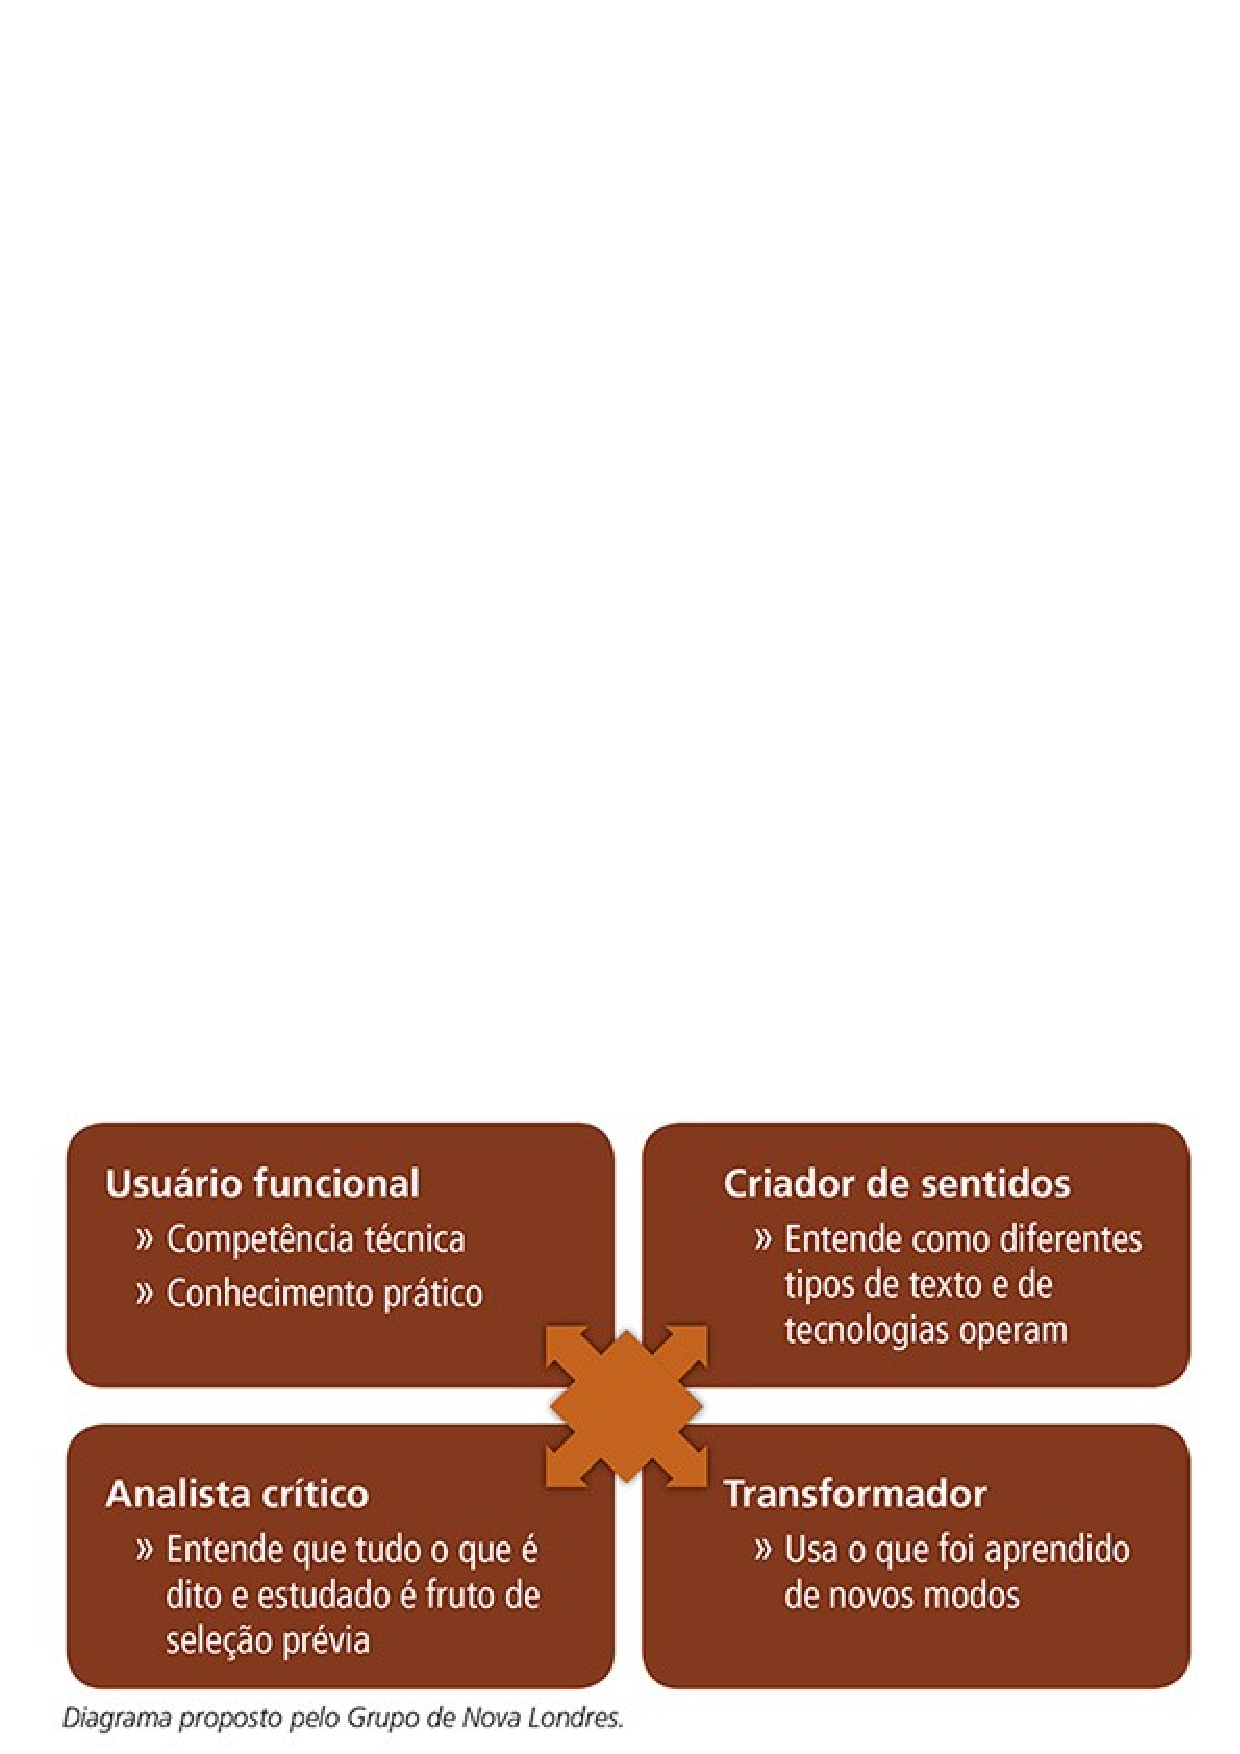
\includegraphics[width=0.5\textwidth]{figure01.pdf}
 \caption{Temática.}
 \label{fig-01}
 \source{elaboración propia.}
\end{figure}

Si contemplamos en el \Cref{fig-02} la categoría gramatical de los nuevos anglicismos en el Diccionario observamos cómo predomina claramente la inclusión de sustantivos con 109 voces. En segundo lugar encontramos 9 adjetivos y, finalmente, 5 verbos. Evidentemente, el predominio de los sustantivos era esperable, ya que, en la transferencia léxica de un idioma a otro, el sustantivo, tradicionalmente, ha sido la categoría gramatical más productiva.

Entre estos sustantivos encontramos un alto número de formas de composición. Observamos los ejemplos de “break dance, chill out, copyriht, fair play, jet lag, playboy, playback, pop art, sex symbol, show business, showman, superwoman, tie break, top model, underground, walkie-talkie, walkman”. Destaca la aparición de anglicismos que contienen el sustantivo “byte”, como en “gigabyte, kilobyte, megabyte, terabyte”.

Dentro de estas categorías gramaticales encontramos fenómenos de adaptación que emplean recursos como la sufijación, la modificación consonántica y la modificación vocálica. En cuanto a la sufijación, se realiza un reajuste ortográfico hacia una forma española. Tenemos el ejemplo del sufijo español de infinitivo “-ar/-ear”: “clicar, cliquear, hackear, tuitear, tunear”. En la transformación del sustantivo o el verbo foráneo en un sustantivo con función de agente encontramos el sufijo “-ero” en “tuitero”. Asimismo, se incluyen adaptaciones con el sufijo sustantivo “-eo” en “cliqueo, tuiteo”.

En cuanto a las modificaciones consonánticas y vocálicas, encontramos un fenómeno recurrente en la ampliación de la forma inicial “s- + consonante” en “es- + consonante”. Observamos los ejemplos de “escúter (scooter)”, “especismo (specism)”, “especista (specism)”, “espanglish (spanglish)”, “espray (spray)”, “esprint (sprint)”, “estand (stand)” y “estriptis/estriptís (striptease)”. Contrariamente, aparece el fenómeno de reducción del grupo final “-ing” por “-in”. Así se incluye “trávelin” en lugar de “travelling”.

Por otro lado, se recurre a la reducción consonántica con los siguientes ejemplos: “ataché” en lugar de “attaché”, “buldócer” en lugar de “bulldozer”, “rocanrol” en lugar de “rock and roll”, “táper” en lugar de “tupper” y “tofe” en lugar de “toffee”.

Incluimos, además, otros fenómenos de sustitución consonántica. En primer lugar, de “q” inicial por “c” inicial con “quark” y “quasar” por “cuark” y “cuásar”. En segundo lugar, de “y” final por “i” en “bioenergía, bodi, brandi, curri, ferri, panti, pinqui” en lugar de “bioenergy, body, brandy, curry, ferry, panty, pinky”.

Finalmente, encontramos voces que mantienen en la adaptación en letra redonda su grafía original, ya que resultan iguales o cercanas a la fisionomía ortográfica de la lengua española. Observamos el ejemplo de “intranet”, que aparece en letra redonda sin transformar sus grafías. Por otro lado, puede suceder que se mantenga la grafía original pero que se añada una tilde para respetar la normativa española de acentuación. De este modo, aparece “bótox” en lugar de “Botox” y “euríbor” en lugar de “euribor”.

\begin{figure}[htbp]
 \centering
 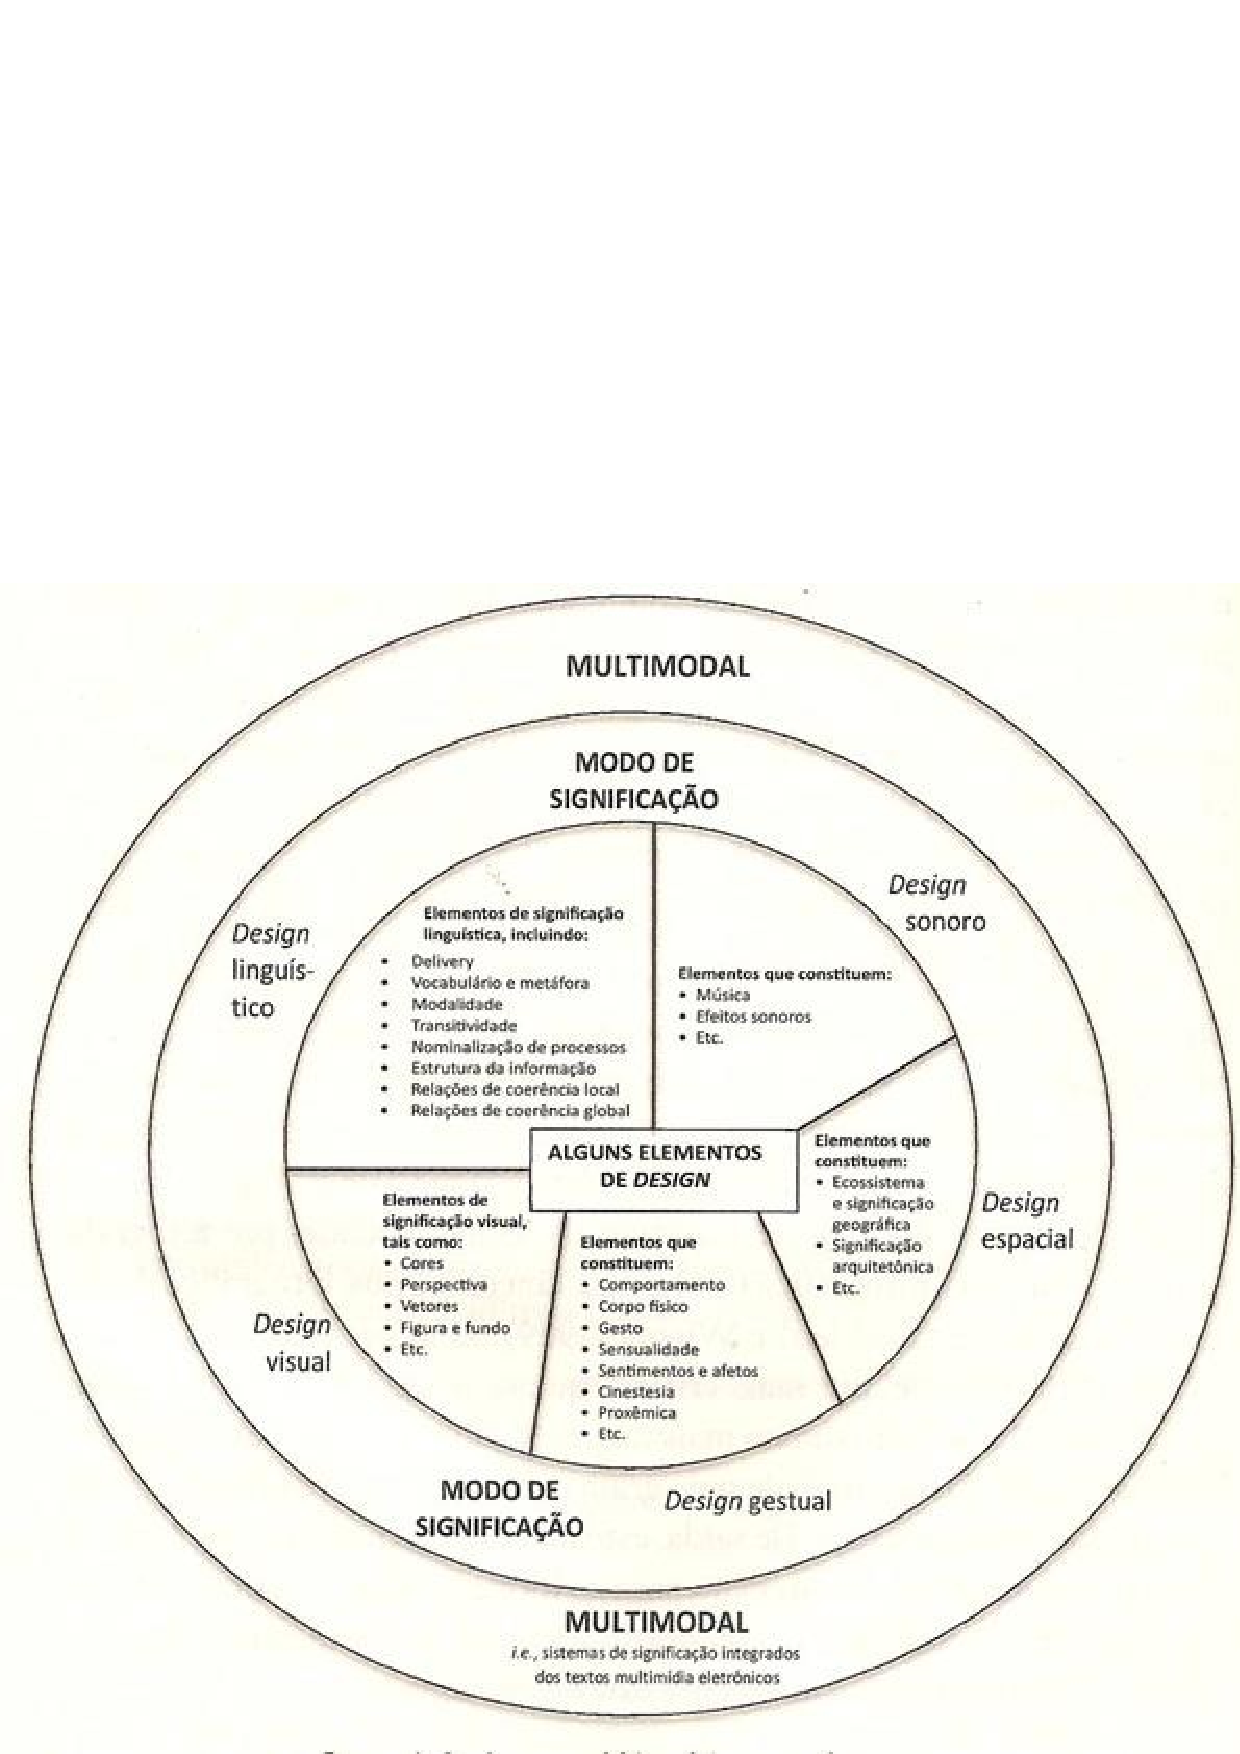
\includegraphics[width=0.5\textwidth]{figure02.pdf}
 \caption{Categoría gramatical de los nuevos anglicismos.}
 \label{fig-02}
 \source{elaboración propia.}
\end{figure}

En cuanto al factor de necesidad de inclusión de las voces (\Cref{fig-03}), encontramos 93 voces necesarias, ya que no cuentan con equivalente en español y, por lo tanto, representan una nueva realidad que necesitaba su correspondiente etiqueta léxica. En segundo lugar, se incluyen 30 anglicismos innecesarios, donde el español sí disponía previamente de una voz que ocupaba el mismo contenido léxico. La mayoría de las voces equivalentes vienen recomendadas por el Diccionario de la lengua española, por lo que se incluye en la Tabla 1 el equivalente propuesto. 

\begin{figure}[htbp]
 \centering
 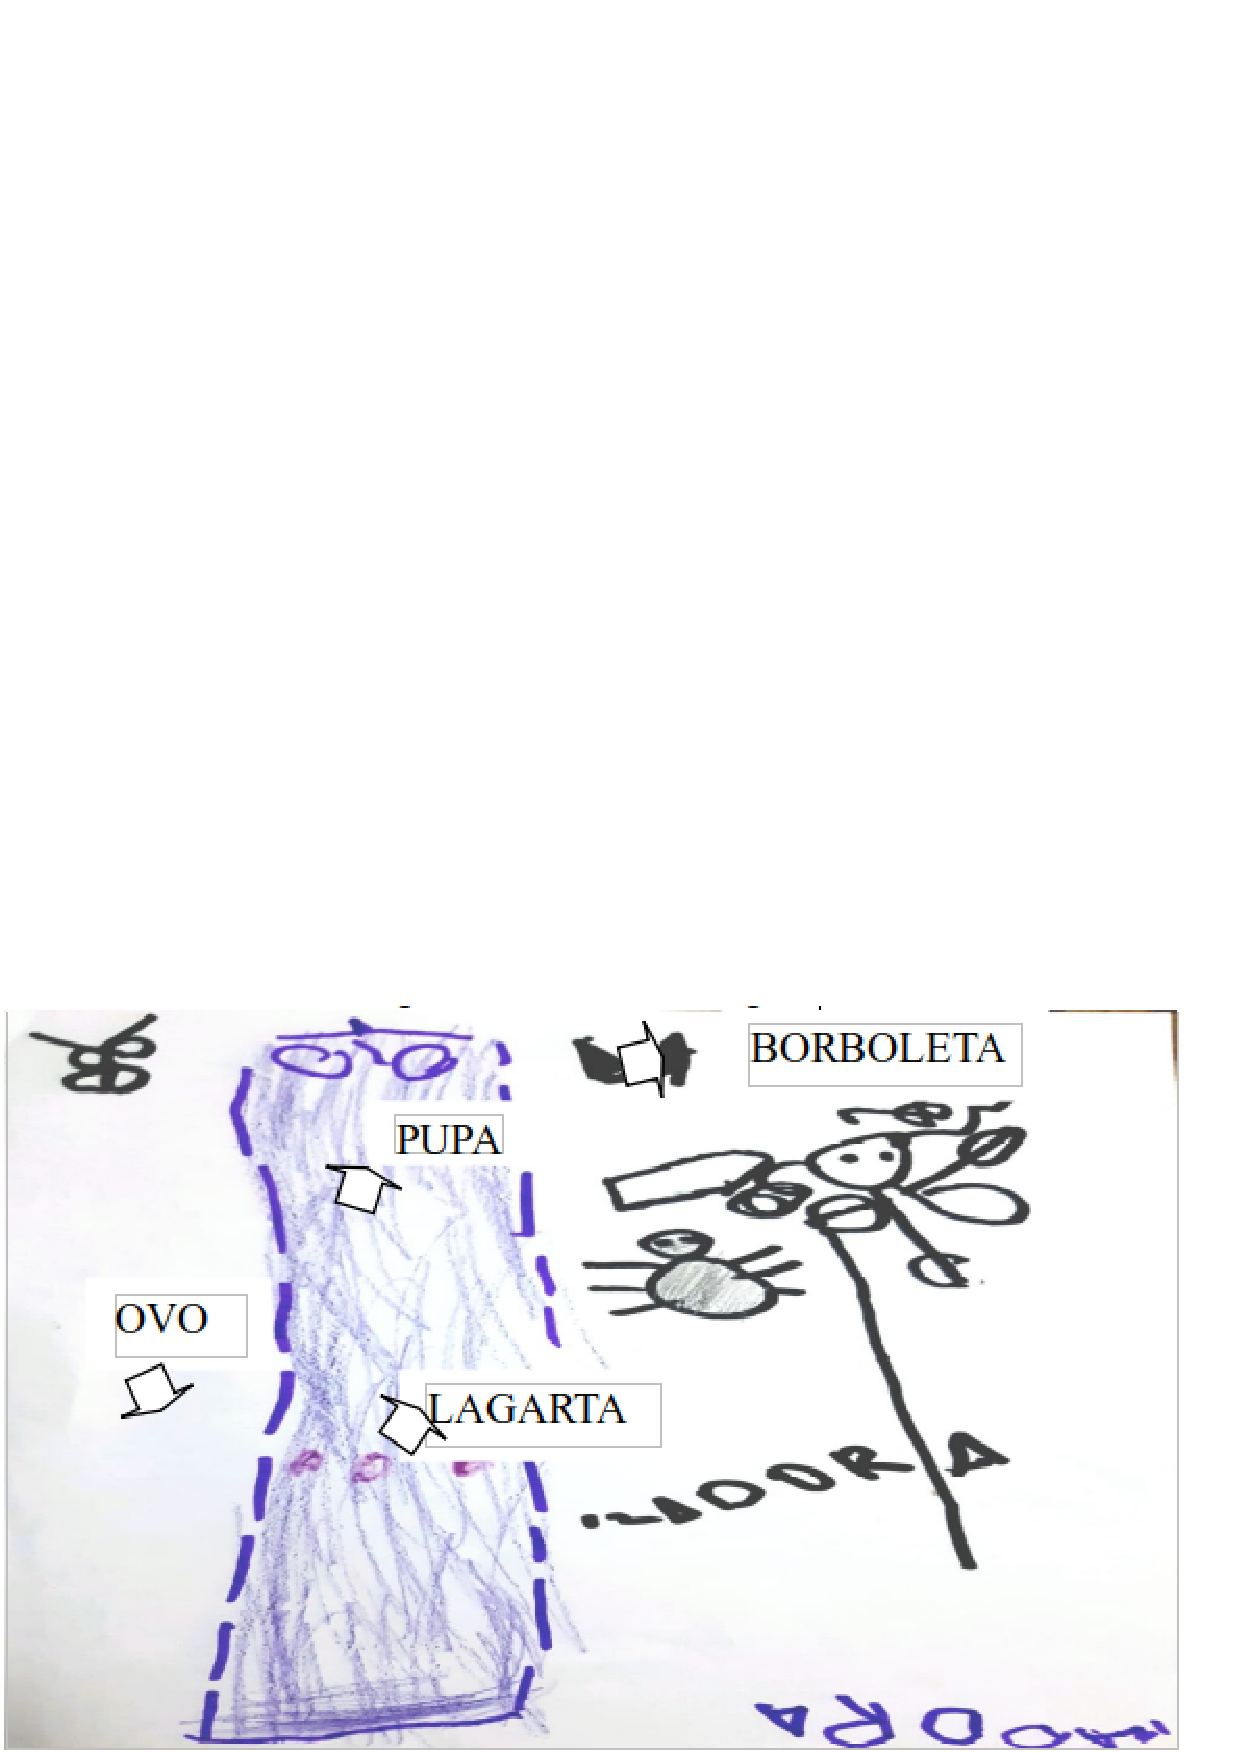
\includegraphics[width=0.5\textwidth]{figure03.pdf}
 \caption{Extranjerismos necesarios e innecesarios.}
 \label{fig-03}
 \source{elaboración propia.}
\end{figure}

Como se muestra en los \Cref{fig-04,fig-05}, observamos que todos los anglicismos tienen mayor frecuencia de uso en CORPES XXI con respecto a CREA\footnote{
También hay que considerar que el CORPES XXI (285.000) recoge más textos que el CREA (111.000).
}. Asimismo, las voces que cuentan con mayor presencia en el CORPES XXI son “performance” (1618), “pub” (1100), “thriller” (933), “coach” (861), “jeep” (742) “spam” (727), “wifi” (693), “stop” (686), “parking” (561), “swing” (557) y “country” (531). Por otro lado, “pinqui” (0), “pinky” (1), “especista” (1) y “especismo” (1) son las voces que tienen una menor representación en el corpus. De este modo, observamos que únicamente la voz “pinqui”, de entre todos los nuevos anglicismos, no tiene presencia en CORPES XXI.


\begin{figure}[htbp]
\begin{minipage}{0.47\textwidth}

\includegraphics[height=4.5cm]{figure04.pdf}
\subcaption{Diez voces con mayor frecuencia de uso en CORPES XXI.}
\label{fig-04}
%\source{elaboración propia.}
\end{minipage}
\hfill
\begin{minipage}{0.47\textwidth}

\includegraphics[height=4.5cm]{figure05.pdf}
\subcaption{Diez voces con menor frecuencia de uso en CORPES XXI.}
\label{fig-05}
%\source{elaboración propia.}
\end{minipage}
\caption{ }
\label{fig-diezvoces}
\source{elaboración propia.}
\end{figure}

Dentro de esta frecuencia de uso, observamos cómo, de todos los nuevos anglicismos, los extranjerismos originales sin adaptación ocupan las primeras posiciones en cuanto a presencia en el CORPUS XXI y, por lo tanto, son los más usados en la sociedad española, siempre según estos textos. Para que el resultado sea significativo, ya que incluimos más anglicismos originales que adaptados en el listado, hemos extraído una media de frecuencia de uso por voz, según se muestra en el \Cref{fig-06}. En el caso de las voces adaptadas la media de frecuencia de uso es de 95,9 apariciones por voz, sin embargo, en el caso de las voces originales en cursiva la media es mucho mayor, de 236,1 por voz.

\begin{figure}[htbp]
 \centering
 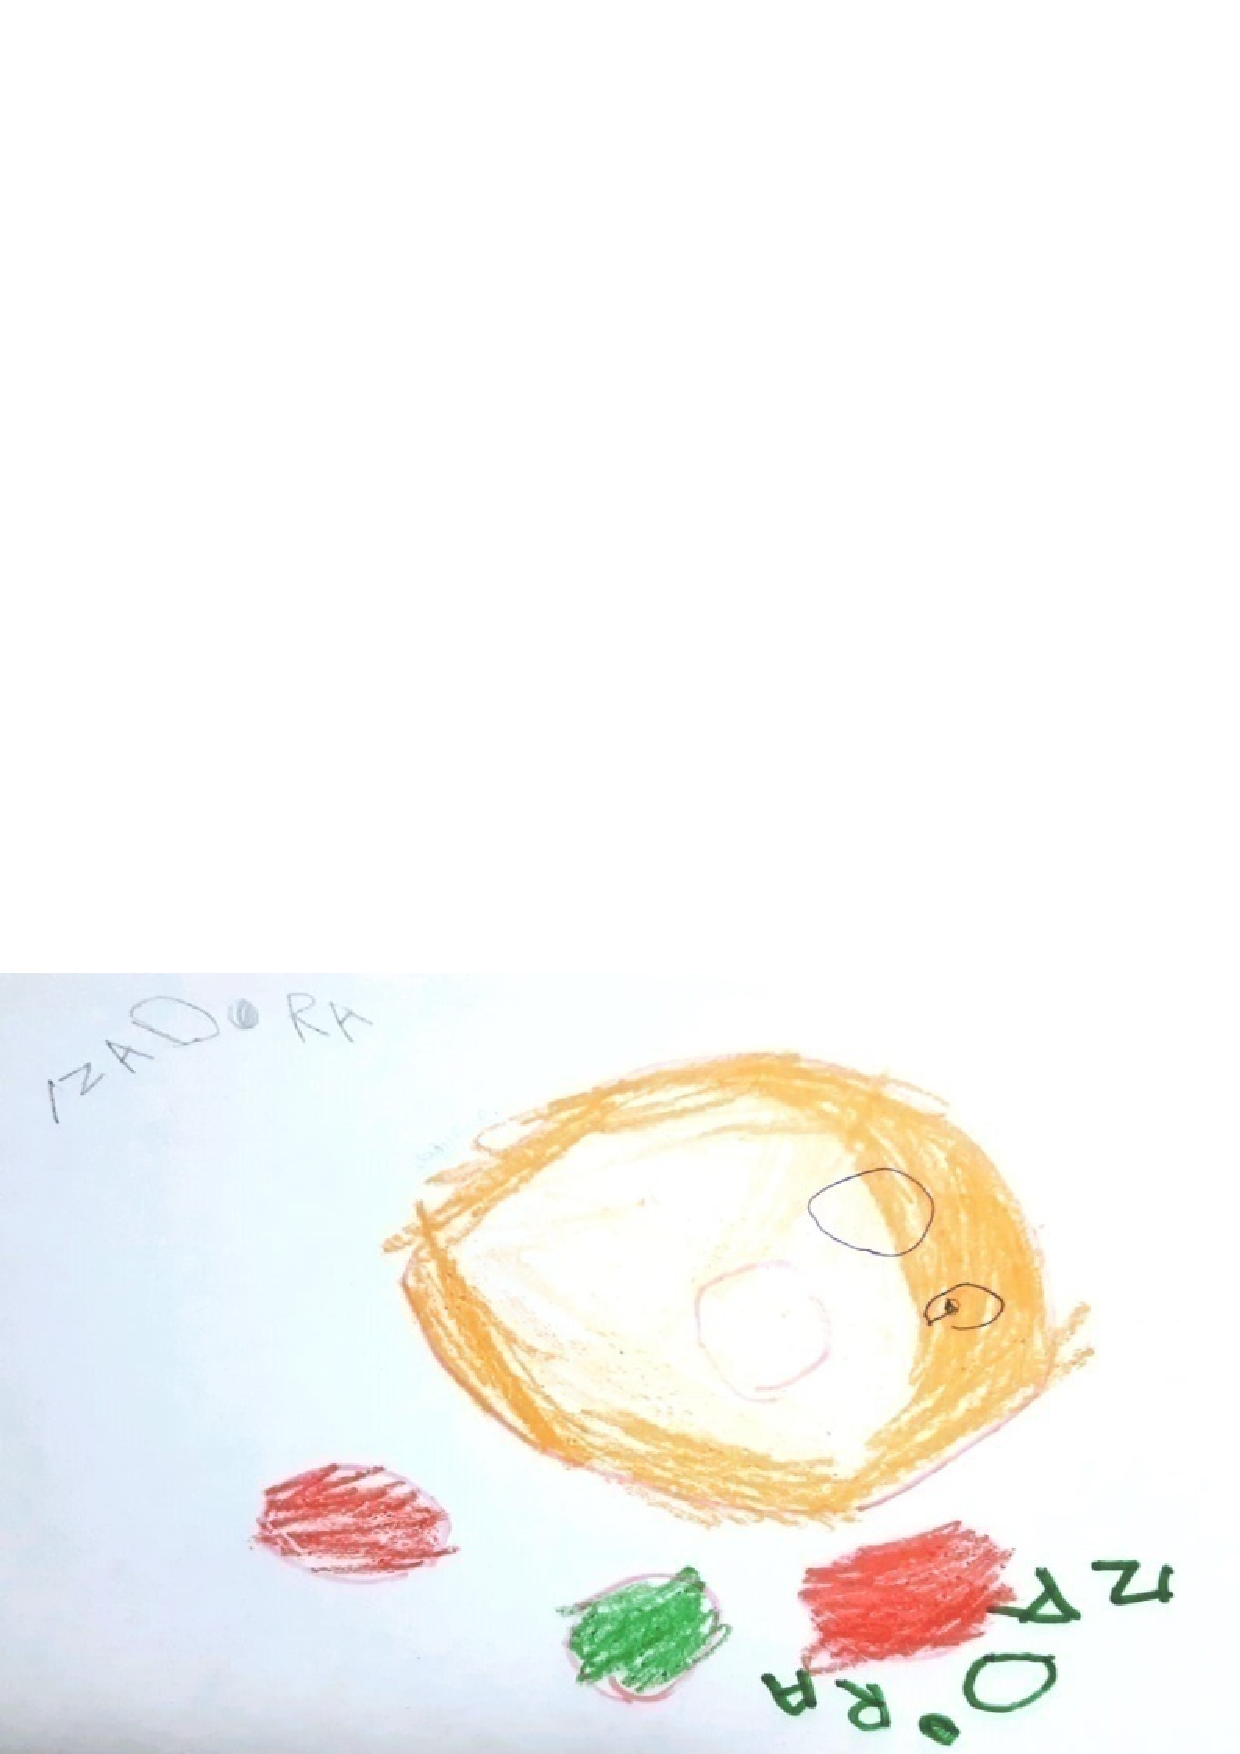
\includegraphics[width=0.5\textwidth]{figure06.pdf}
 \caption{Media de frecuencia de uso en voces originales y adaptadas en CORPES XXI.}
 \label{fig-06}
 \source{elaboración propia.}
\end{figure}



\section{Conclusiones}\label{sec-conclusiones}
Como hemos podido apreciar, la llegada de nuevos anglicismos a la lengua española es un hecho que se ve representado en los corpus y diccionarios académicos. En esta investigación hemos incluido y analizado 123 nuevos anglicismos en el DLE (23.ª edición) en relación con su edición anterior (22.ª edición). Resulta un número considerable de voces para una sola edición de diferencia, hecho que, asimismo, nos haría replantear esa concepción purista que desprende la RAE en la sociedad con respecto a la inclusión de extranjerismos. Pese a que es cierto que este organismo académico realiza una campaña a favor de las voces patrimoniales, este factor no evita que edición tras edición se incluya un notable número de anglicismos que reflejan su uso social en los textos escritos y orales del español, principalmente en las últimas décadas. Por lo tanto, tendríamos que hablar más acertadamente de un criterio equilibrado y controlado a la hora de incorporar anglicismos, ya que, tal y como hemos demostrado, se requiere del parámetro de frecuencia de uso en los corpus académicos, en concreto, en CORPES XXI, herramienta académica actual.

En cuanto a la tipología de estas voces, observamos cómo el prototipo de anglicismos que prefieren incluir la RAE y la ASALE es el del anglicismo original en cursiva que, además, no disponga de un equivalente patrimonial. De este modo, queda clara la postura de recoger, principalmente, aquellas voces que resulten necesarias y que no puedan obstaculizar el uso de una voz patrimonial, por lo que se muestra una mayor resistencia hacia las voces innecesarias, lo que demuestra su baja inclusión. De hecho, en los anglicismos que sí disponen de este equivalente, se señala la preferencia por la voz patrimonial, como ya se indicaba en el Diccionario panhispánico de dudas y como se sigue poniendo de relieve en las diferentes ediciones del DLE. Otro factor que nos indica que realmente se sigue el uso social de estos anglicismos queda patente en que los extranjerismos originales en cursiva son los que tienen una media de uso más alta en la sociedad hispanohablante, que paralelamente coincide con el hecho de que sean las voces que mayor número de inclusión tienen en el Diccionario, en detrimento de las voces adaptadas.

Por otro lado, en las voces adaptadas en letra redonda observamos el objetivo que guardan la RAE y la ASALE de asimilar y, dentro de lo posible, “españolizar” las voces extranjeras. Mediante mecanismos de derivación y sustitución consonántica y vocálica, este organismo intenta evitar aquellas formas ortográficas que resulten ajenas al español. Ejemplos recurrentes desde la voz inglesa al español resultarían la sustitución de “-in” por “-ing”, la ampliación del grupo inicial “s + consonante” a favor de “es + consonante” o las sustituciones de los dígrafos “tt”, “pp”, “ff” en favor de la grafía simple.

Pese a que muchos de estos anglicismos ya aparecían en el corpus CREA durante los años 80 y 90, aumentan su frecuencia de uso durante los primeros años del siglo XXI, como observamos en el CORPES XXI, y es, por lo tanto, en la última edición del Diccionario \cite{real2014diccionario} cuando la RAE y la ASALE se deciden a incluirlos. Además de la progresiva apertura comunicativa y el mayor intercambio lingüístico que experimenta la sociedad y que provoca que cada vez aumente más el número de voces de otros idiomas que son conocidas por los hablantes.

En definitiva, hemos podido observar que el factor de frecuencia resulta fundamental para que un anglicismo se añada a esta nueva edición del Diccionario académico, ya que, a excepción de “pinqui”, cuya voz original “pinky” sí cuenta con presencia, todos aparecen en el CORPES XXI. En cualquier caso, este factor no es definitivo, ya que se contemplan otros criterios como la necesidad de la voz en el vocabulario español o su adaptabilidad a este idioma. De hecho, si simplemente el factor de frecuencia de uso fuera el requisito para formar parte de las obras lexicográficas académicas, voces como “influencer, online, tablet, follower, like, link, streaming, spin-off”, todos ellos anglicismos con una gran presencia en el CORPES XXI, deberían aparecer en estas obras. El motivo que esgrimen la RAE y la ASALE, hasta el momento, es que los equivalentes patrimoniales todavía tienen vigencia y se recomienda su uso, de ahí a la importancia del factor de necesidad: “influyente, en línea, tableta, seguidor, me gusta, enlace, en directo, serie derivada”. No obstante, siguen siendo voces de amplio uso y extensión internacional. Por lo tanto, en esta situación dinámica de contacto lingüístico como la que estamos viviendo, tendremos que estar atentos a la creciente llegada de anglicismos a la lengua española y a los criterios generales y puntuales, en ocasiones confusos, de frecuencia de uso, necesidad y capacidad de adaptación que siguen empleando los organismos académicos.



\section*{Financiamiento}
Este trabajo se enmarca en el proyecto La atenuación pragmática en su variación genérica: géneros discursivos escritos y orales en el español de España y América (FFI2016-75249-P), financiado por el Ministerio de Economía y Competitividad de España.




\printbibliography\label{sec-bib}


\end{document}
